

% Laatu painottuu startupissa siihen, mitä asiakkaat ja loppukäyttäjät pitävät tärkeänä
% Laadun merkitys elinkaaren eri vaiheissa muuttuu
%	-Aluksi tärkeintä validoida featuret ja idea
%	-Laadussa tärkeää aluksi hyvä muokattavuus, refaktoroinnit, asiakkaalle kriittisten osien testaus
%	-Elinkaaren alussa ei väliä matalan prioriteetin bugeilla tai featureiden vajaalla toiminnalla
%	-Kun idea alkaa olla validoitu, muuttuu laadun merkitys tuotteistuksen yhteydessä
%	-Laatuun on käytössä myöhemmin enemmän resursseja, koska asiakkaita alkaa olla
%	-Osuiskohan tähän Lean Startupin skaalausvaihe

 \section{Evaluation of QA Methods}

Quality assurance in a startup environment differs from the QA activities in traditional software development. This is because the requirements and goals of a startup project are usually considerably different from a traditional software projects. Furthermore, even the term software quality can be partially redefined for a better fit in a software startup. Eric Ries describes that the development of Minimum Viable Products questions the traditional notions of quality and this is the most vexing aspects of the development. TODO: Viite

 \subsection{Quality in a Startup project}

In the beginning of the chapter about role of quality, Eric Ries states that "The best professionals and craftpersons alike aspire to build quality products; it is a point of pride". This is a good summary about the attitude towards software quality in many movements about modern software development. Measuring and defining quality in modern software projects with constant changes and uncertainty can be difficult, but the development personnel should have the pursuit for high quality.

Ries tells that modern production processes seek to boost efficiency by relying to high quality. The belief that the customer is the most important part of the production process means that all effort should be focused to producing results that the customer finds valuable. This view can be beneficial in an environment where the company knows the opinions of customers. However, in a startup development, assuming the opinions of customers is a risky thing to do. Often in the startup, it is not even sure who the customer is. Thus, Ries introduces a quality principle for startups: "If we do not know who the customer is, we do not know what quality is".

In a startup developing an MVP, the quality of the product can be a fluid concept. Even if the quality of MVP is low for customers, it can bring great value in building a high-quality product. If the customers find the product low on quality, this can be used as an opportunity to learn what customers care about. This is infinitely better than mere speculation, because it provides empirical information on which to build future products.

When working with a 3D chat software called IMVU, Ries and his colleagues decided to leave a critical sophisticated feature done with only minimum effort. They were embarrassed to release the moving of the avatars without any animations or other modern visualizations. The avatars just reappeared to another location. The response of the customers was surprising as the customers were thrilled from the new feature, which allowed an immediate change of location without waiting. From the customers point of view, the released feature was more appropriate than the option which would take more time and money to implement. In the end, the quality of the released feature was probably higher than the one planned. The lesson behind the story is that customers do not care how much time something takes to build.

Lean Startup method is aiming for the goal of winning over customers and not opposed to building high-quality products. Thus, it is necessary to set aside some professional standards to enable the validated learning as soon as possible. This is not supposed to allow operating in an undisciplined manner. This is important as there are some quality problems that can slow down the Build-Measure-Learn feedback loop. In addition, defects complicate the evolution of the product and interfere with the ability to learn. Helping the development of the MVP means removing any feature, process or effort that does not lead directly to the learning sought.~\cite{ries2011lean}

\subsection{TODO: Foundations of high quality}

 \textbf{Clean code.} Every programmer with experience for more than two or three years have probably been slowed down by messy code. Over a couple of years of development, teams that were moving fast at the beginning of the project can be slowed down to a really slow pace. Development begins to include more and more non-trivial changes, which are about resolving the existing knots and tangles and adding new. Eventually, the mess can become so big that it can not be cleaned up at all. The total cost of owning a mess is being pondered by Robert C. Martin in his book Clean Code: A Handbook of Agile Software Craftmanship.

 Martin reminds that "code is really the language in which we ultimately express the requirements" and thus code is in the very foundations of every software project. A common mistake done in software projects is to increase the measure of developers in the team. This is usually done when the code has already reached a too messy state and the pace of development has slowed down. Adding new staff to the development does not improve the situation, but underlines the meaning of messy code. This new staff is not familiar with the existing system, so they easily complicate the system even further, driving the productivity even worse.

 A bitter fact for the developers is that usually the cause of messy code is the fault of the developers. While the management and sales staff are defending schedules and requirements, the developers should be defending the code. Many developers previously slowed down by messy code still feel the pressure of deadlines and the temptation to make messes to achieve them. Martin says that true professionals know that the only way to go fast is to keep the code as clean as possible at all times. A programmer able to write clean code is an artist, who can use all the little techniques in a disciplined manner through the sense of cleanliness.~\cite{martin2008clean}
 
 \textbf{Integrity.} One of the principles of Lean Software Development (LSD) is "Build Integrity In", which has its premises in high-performing automotive companies in 1980s. A study "Product Development Performance" by Kim Clark found out that the product integrity was a key difference between average and high-performing companies in developing superior products. Clark found out that integrity has two dimensions: external integrity and internal integrity.~\cite{clark1991product}

 LSD renames these two types of integrities as perceived integrity and conceptual integrity. Perceived integrity is a balance of function, usability, reliability and economy observed by the customer. It is affected by the whole experience of the system beginning from advertising and delivery to intuitiveness and the ability to solve the problem. An analogy to the measure of perceived integrity comes from the question: which ones of the bookmarks of your browser would you add back immediately, if you wiped out them all? These are the products with perceived integrity. 

 Conceptual integrity is smoothness and uniformity of the whole system's central concepts. The architecture of the system has an effective balance between flexibility, maintainability, efficiency and responsiveness. Conceptual integrity is a prerequisite to perceived integrity. To be able to achieve perceived integrity, the system must have a consistent design. As the system evolves and matures, conceptual integrity emerges. Although conceptual integrity is needed for perceived integrity, the existence of the former does not ensure the existence of the latter. This is because conceptual integrity is not sufficient for a successful customer experience, if the system does not meet the users' need.~\cite{poppendieck2003LSD}

\subsection{TODO: Aiming towards high quality}

\textbf{Build Integrity In.} In the study by Kim Clark, a primary claim is that integrity is achieved through superior information flow. Perceived integrity is a projection of the integrity of the information flow between users and developers. In turn, conceptual integrity is a projection of the integrity of the upstream and downstream of technical information flow. When reaching a system with high perceived and conceptual integrity, an excellent information flow is necessary both between customer and development team and between the upstream and downstream processes of the development team. Information flows must take into account both the current and potential uses of the system.

% Perceived integrity
In traditional software development, perceived integrity is transmitted to programmers through a multistage process. In this process, requirements are collected and processed through analysis and design. Then the design is transfered to the programmers implementing the code. These multiple hand-offs will cause the loss of considerable amount of information, key details and future perspectives. Fortunately, an alternative for this multistage process is to establish a superior customer-developer information flow by other means. With smaller systems, the development should be done by a single team having direct access to the people capable of judging the systems integrity. This team should use short iterations in where the system is demonstrated to a wide range of people giving feedback about the integrity. This way the feedback can be used for a rapid steering of course. Another technique is to use customer tests purposely created for getting feedback.

% Conceptual integrity
% Communicating two-ways face to face in small batches and solving the problems at the same time
Conceptual integrity in automotive manufacturing is pursued by using existing parts and integrated problem solving. In integrated problem solving, understanding and solving the problem happen simultaneously, instead of sequentially. The initial information is released early and not only after complete information is available. Information flow happens in two directions instead of one and it contains multiple small batches of information instead of a single large batch. The preferred communication style is face to face instead of documents. This kind of problem-solving is ideal for achieving conceptual product integrity, particularly in development of complex systems such as automobiles or software systems.

In software development, using integrated problem solving means that the development must be started before the design is finalized. In addition, the developers should be able to access customers or customer representatives for getting the answers as soon as possible for any questions raised. Customer tests should be developed and ran along the iterations and not just at the end.

Finally, using experienced developers in their own areas of expertise can help in achieving conceptual integrity. Not all of the developers have to be with plenty of experience, but for the complex areas, experience brings understanding of the technical details and patterns widely used to manage with the complexities. One of these experienced developers should be a master developer facilitating the effort over multiple teams. For example, integrating the decisions and trade-offs among multiple developers and customers would be the responsibility of the master developer.

% Refactoring
When the integrity of a product is building, the iterative development brings continuous improvement as the product is evolving. In software development, the system must be continuously improved by the developers. Otherwise the internal structures of the software will become calcified and fragile. In time, the system will even stop working. Refactoring is done to prevent this disintegration of the software structures over the development.

The need for refactoring comes when new features are added to the system one at a time and the architecture and requirements of the system change gradually. Often it would be better to think of new related features as a set and build an architectural capability to support them. If the features are added in multiple different locations of the code, the system will lose conceptual integrity. Refactoring regularly keeps the system healthy.

TODO: p. 142-144

% Testing
In a traditional software development implementing single module at a time, there are numerous types of testing used. There are for example unit testing, system testing, integration testing and acceptance testing used. The purpose of testing is to check that the intention behind the design is achieved and the system does what the customers want it to. In LSD, the development is done by implementing entire features instead of single modules, so the distinction between the different kinds of testing types is more artificial. Instead, testing is divided into two parts: developer tests and customer tests. Developer tests are testing that the implemented features work as intended and that all the pieces work together. In turn, customer tests are developed to verify that the system does what customers expect.

%	Developer tests: unit, system, integration 
%	Customer tests: acceptance tests
%	Communication
%	Feedback
%	Scaffolding

% LSD: design cycles, right the first time, cycles involving business
% Frequent problem-solving cycles spanning upstream and downstream engineers

\textbf{Empower the Team.}



% \textbf{TDD.}

\textbf{Iterative development.}

\textbf{Activities.}

\begin{figure}[t]
\begin{center}
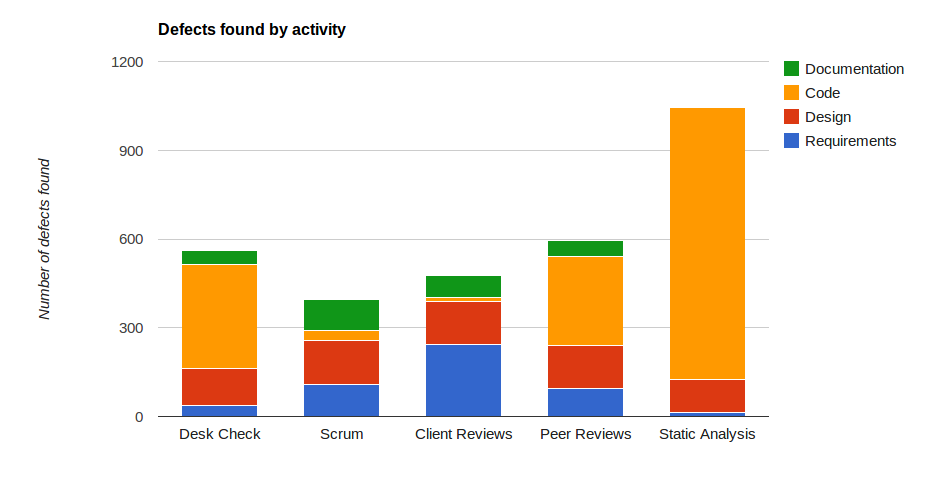
\includegraphics[width=1.0\textwidth]{image/pretest-efficiency.png}
\end{center}
\caption{Efficiency of pretest defect prevention}
\label{fig:pretest-efficiency}
\end{figure}

Figure~\ref{fig:pretest-efficiency}

% PREVENTIVE
% -Small business applications p.126
% 	-1000fp
% 	-embedded users
% 	-agile development method
% 	-TDD
% 	-automated risk analysis
% 	-static analysis on all code segments
% -This combination should lower defect potentials by 45\% and ensure defect removal 95\%

% ECO: We use these quality metrics to compare a number of quality improvement techniques at each stage of the software development life cycle and quantify their efficacy using data from real-world applications.
 
% Direct costs \& efforts p. 200 table
% ECO: Analysis of pretest defect removal activities p. 208
 
% DEFECT TRACKING IS A WASTE

%http://books.google.fi/books?id=RTt9AgAAQBAJ&lpg=PA27&ots=PXXKjr2e_E&dq=%22According%20to%20Shigeo%20Shingo%2C%20there%20are%20two%20kinds%20of%20inspection%22&pg=PA29#v=onepage&q&f=false
% In Lean Software Development, the goal is to build quality into the code from the start, not test it in later. Dont focus on putting defects into a tracking system, you avoid creating defects in the first place. It takes a higly disciplined organization to do that. p26
% There are two kinds of inspections, inspection after defects occur and inspection to prevent defects. If you really want quality, you don't inspect after the fact, you control conditions so as not to allow defects in the first place. If this is not possible, the you inspect the product after each small stemp, so that defects are caught immediately after they occur. When a defect is found, you stop the line, find its cause and fix it immediately. p.27
% Defect tracking systems are queues of partially done work, queues of rework. In Lean, queues are collection points for waste.

% {poppendieck2006implementing} 

\subsection{The Don'ts - Things To Avoid}
 
% \begin{itemize}
 
% Liittyy vahvasti Leanin Wasteen
% Älä raportoi bugeja, joista tiedät, ettei niitä korjata
% Ei turhia raportteja
% ECO: Cost per defect => paras tulos bugisimmassa projektissa
 
% \end{itemize}

% ECO:  p. 127 harmful combinations PREVENTIVE

Capers Jones has interpreted from the research of multiple years of software quality that there can be harmful combinations of methods used. Even when combinind harmful methods with helpful ones, the harmful method seem to end up winning. That is, defect potentials are raising instead of coming down. Some methods combined with others can raise the defect potentials and make applications risky with a change of failure.
